\documentclass[10pt,a4paper]{article}
\usepackage[utf8]{inputenc}
\usepackage[german]{babel}
\usepackage[T1]{fontenc}
\usepackage{amsmath}
\usepackage{amsfonts}
\usepackage{amssymb}
\usepackage{graphicx}
\usepackage{caption}

\DeclareCaptionFormat{citation}{%
   \ifx\captioncitation\relax\relax\else
     \captioncitation\par
   \fi
   #1#2#3\par}
\newcommand*\setcaptioncitation[1]{\def\captioncitation{\textit{Quelle:}~#1}}
\let\captioncitation\relax
\captionsetup{format=citation,justification=centering}

\author{Manuel Rickli, Lukas Stöckli, Michael Plüss}
\title{LED Bank}
\begin{document}
\maketitle

\section{Einleitung}

Das Ziel unserer Gruppe war, eine LED Bank zu bauen. Diese besteht aus 48x8 grünen LEDs, welche als Pixel fungieren. Darauf soll man kurze Texte anzeigen können, welche von rechts nach links scrollen. Die LED Bank soll sich mit dem Internet verbinden können und Pixeldaten von dort entnehmen und anzeigen.\\
Die Vision ist, diese LED Bank im Zimmer aufhängen oder hinstellen zu können und darauf verschiedenste Informationen darzustellen. Es sind auch Anwendungen wie eine Uhr, eine Wetterangabe geplant oder sogar kleine 48x8 Pixel Filmchen.\\

\section{Hauptteil}

\subsection{Umsetzung}

\subsubsection{Display}

!!!!!!!!!!!!!!!!!!!!!!!!!!!!!!!!!! TODO!!!!!\\
(Bild)\\\\

Die 384 LEDs befinden sich verteilt auf zwei Steckbrettern. Die acht Reihen der Bank werden direkt vom Arduino angesprochen. Die 48 Kolonnen steuern wir über drei Pins des Arduinos mittels Schieberegister. Ein Schieberegister hat jeweils acht Output Pins, weshalb wir insgesamt sechs davon benutzen, welche in Reihe geschaltet sind.\\
Wir erreichen die Darstellung eines komplexen Pixelmusters, indem wir jeweils die Pixeldaten der Zeile in die Schieberegister einfüttern und dann den dazugehörigen Pin einschalten. So wird jeweils eine horizontale Linie dargestellt. Diese lassen wir einen kurzen Moment leuchten und gehen dann zur nächsten Zeile über. Wenn wir alle Zeilen dargestellt haben, haben wir ein Frame 'gezeichnet'. Mit einer genug schnellen Taktrate wirkt es für das menschliche Auge so, als würden die LEDs dauernd leuchten.\\

\subsubsection{Code}

Der Code für das Arduino haben wir in der Arduino IDE geschrieben und bildet die Kontrolle über den Display, sowie die Kommunikationsstelle zum Internet.\\
Um Texte darstellen zu können haben wir viele Bitmuster für die einzelnen Buchstaben einprogrammiert, welche auf unsere Bedüftnisse angepasst sind.\\

\subsubsection{Webseite}

Auf dem Arduino läuft ein kleiner Webserver, der eine Konsole zur Verfügung stellt. Der Server schickt dem Client HTML Code, den der Browser dann in die sichtbare Website umwandelt. Über ein Eingabefeld kann Text an den Server übergeben werden, der dann auf der LED-Matrix angezeigt wird.

\subsection{Technische Details}

\subsubsection{Display}

Wir haben für unsere Anzeige folgende Bauteile verwendet:

\begin{itemize}
\item LED 20mA, 2,2V
\item Widerstand 3.3k$\Omega$
\item Widerstand 220$\Omega$
\item Schieberegister 74HC595
\item Transistor Array ULN2803
\item Kondensator 1$\mu$F
\end{itemize}

Da die LED's mit 20mA betrieben werden sollte und  \[R = 5V/20mA = 250\Omega\] haben wir 220$\Omega$ Widerstände als Vorwiderstand eingebaut. Der Strom wäre leicht höher als 20mA, die 5V des Arduino erreichen jedoch auch nicht ganz die Anzeige aufgrund von Spannungsabfall. Diese Vorwiderstände befinden sich zwischen den Schieberegistern und den LED-Kolumnen. Die Reihen werden direkt über das Arduino angesteuert. Da dieses bei den Output-Pins jedoch nur ca. 40mA gesourced oder gesinkt werden können, wird der ULN2803 dazwischen geschaltet. Diesen kann man bis 500mA und 50V betreiben. Davor wird für jede Reihe ein 3.3k$\Omega$ Widerstand geschaltet, da über die Leitungen vom Arduino nur noch Impulse an den ULN2803 gesendet werden, welche diesen dann zum Schalten bringen. Die ganze Energie kommt also direkt von Ground und 5V und nicht über die digitalen Outputs des Arduino.

Auf dem Schieberegister hat man Ground, 5V und die acht Ausgänge. Zusätzlich, um die Schieberegister anzusteuern, benötigt man drei Verbindungen zum Arduino:
\begin{itemize}
\item Latch Pin
\item Clock Pin
\item Data Pin
\end{itemize}

Der Clock Pin bestimmt, wann über den Data Pin die Register beschrieben werden. Nur wenn dieser auf HIGH geschaltet wird, können die im Data Pin gespeicherten Bytes gesendet werden. Ist der Latch Pin auf HIGH, so werden die im Register gespeicherten Reihen mit Spannung versorgt. Deshalb muss vor dem Neubeschreiben dieser auf LOW gesetzt werden. In unserem Falle geben wir mit jedem shiftOut() genau ein Byte mit. Dieses wird immer in dem ersten Register gespeichert. Ist es schon beschrieben, so wird dieses Byte an das nächste Register weitergegeben. Wir rufen also sechs mal shiftOut() auf und geben als erstes Byte die Information für das sechste Register mit.

\begin{figure}
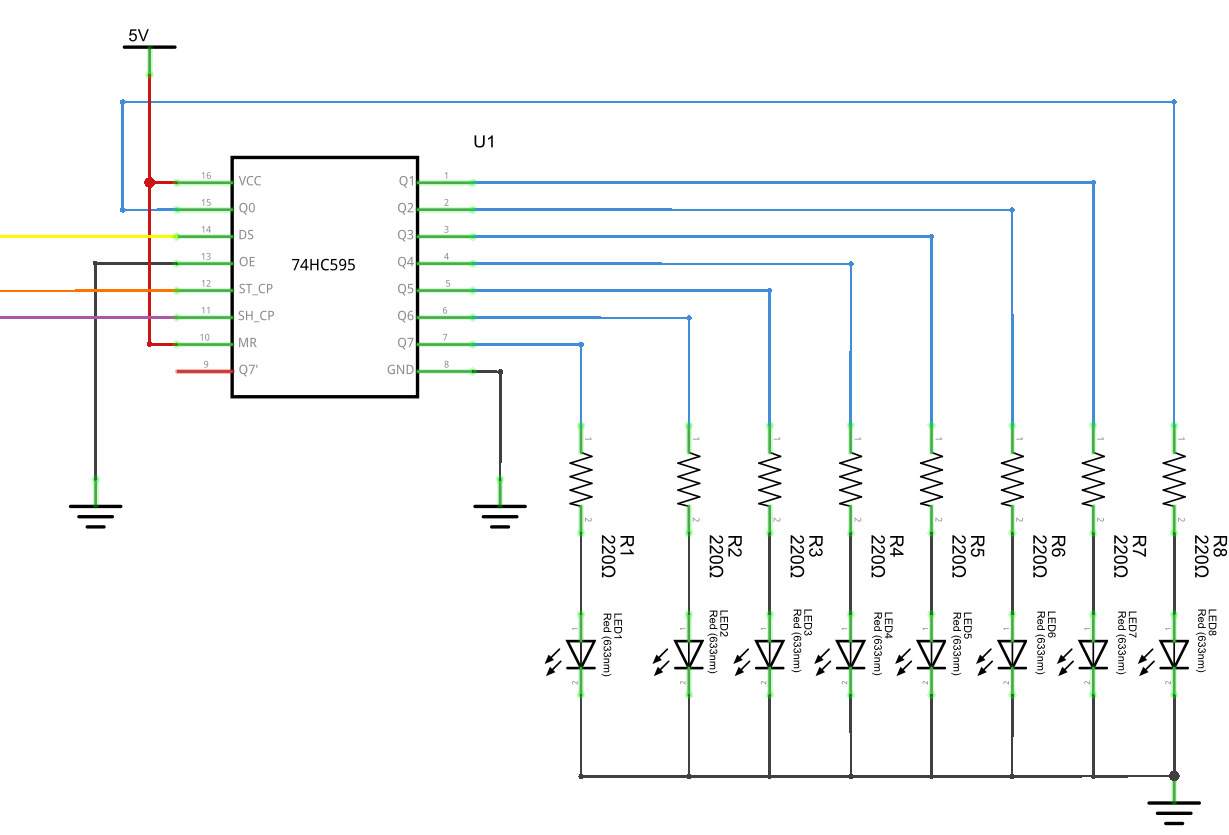
\includegraphics[width=\textwidth]{shiftReg.png}
\setcaptioncitation{arduinolearning.com/learning/basics/interfacing-74hc595.php}
\caption{Schema vom 74HC595 mit LEDs am Ausgang}
\end{figure}

\subsubsection{Code}

Der Code ist in verschiedene Module unterteilt, die zusammen die Funktionalität des Produkts gewährleisten.

Das 'main' Modul initialisiert die restlichen Module und enthält den Mainloop, in dem die Frames gezeichnet werden, die Laufschrift aktualisiert wird und der Server betrieben wird.

Das Modul 'internetInterface' ist verantworlich für die Internetanbindung unseres Systems. Es besteht aus dem Requesthandler und einem Setup-Modul, das die physische Verbindung initialisiert und den Server startet. Der Requesthandler sendet den Code für das Anzeigen der Webseite und bearbeitet die Eingaben, welche über die Console eingehen, um den Text zu ändern.

Das Modul 'ledInterface' hält den Grafikspeicher, welcher aus einem 48x8 Char-Array besteht. Dieses speichert die Lichtzustände der Pixel. Das Modul enthält ausserdem die Methoden zur Textbearbeitung und ist verantwortlich für das Übersetzen von Usereingaben in die Bitmap, sowie das aktualisieren der Laufschrift. Hier werden Buchstaben in Arrays mit 8-Bit Zahlen umgewandelt.

Das Modul 'chars' hält die ganzen Informationen über die darstellbaren Zeichen. Dies sind einerseits die Bitmap und andererseits die anzuzeigende Breite.

Als letztes gibt es das Modul 'ledHardwareControl'. Es ist verantwortlich für die Anzeige des Grafikspeichers auf der LED-Matrix. Über die Pins des Arduinos werden Reihen und Spalten angesprochen um das gewünschte Frame anzuzeigen.

\subsubsection{Webseite}

Auf dem Arduino läuft ein Webserver mit einer Internetseite. Über die IP 192.168.178.42 und den Port 80 kann darauf zugegriffen werden. Die Webseite enthält ein Feld, um einen neuen Text auf die Anzeige zu laden. Der Requesthandler schickt den HTML/CSS Code an den Client. Falls er vom Client einen Request bekommt, wird keine Seite gesendet. Stattdessen untersucht der Parser die Nachricht und aktualisiert die Anzeige.

\section{Zusammenfassung}

Insgesamt war die LED Bank ein Projekt überschaubarer Komplexität. Darauf hatten wir auch abgezielt. Da wir anfangs alle nicht so erfahren waren im Löten, mussten wir zuerst etwas den Einstieg finden. Dies führte dazu, dass wir mehrere Lötstellen im Nachhinein reparieren mussten. Schwieriger als erwartet, war der Umgang mit den Schieberegistern, welche sich Anfangs nie so verhalten haben, wie wir es geplant hatten. Auch mühsamer als erwartet war die Verbindung des Arduinos mit dem Internet. Der Schwerpunkt lag eher auf Seiten der Hardware, da wir alles selbst zusammenstellten und verlöteten. Schlussendlich war es ein tolles Gefühl, als unsere Hardware das tat was sie sollte. Auch Softwaretechnisch haben wir unser Ziel erreicht und planen jetzt schon weitere Funktionen.

\end{document}